% FILLED (fill batch): process ① Production — pair-production threshold.
%   folds stdlib pair_threshold_* kinematics + Chamberlain–Segrè 1955 Bevatron
%   design number + verify atoms pair_threshold_factor / _kinetic / _total +
%   the BLUE-MAX integer factors 6/7, from companion/verify-ledger.json.
\section{Production --- Pair-Production Threshold Kinematics}
\label{app:production}

This appendix is the full data record for pipeline process
\textcircled{\scriptsize 1}. We derive the fixed-target pair-production
threshold $p+p\to p+p+\bar p+p$ from lab-frame four-momentum conservation,
giving the exact integer relations $T_{\mathrm{th}}=6\,m_pc^2$ (beam kinetic)
and $E_{\mathrm{beam,th}}=7\,m_pc^2\approx6.5$\,GeV --- the historical
Bevatron design number that produced the first antiprotons
\citep{chamberlain1955} --- and trace every digit to the verify atoms in
\texttt{companion/verify-ledger.json}.

% -------------------------------------------------------------------------
\subsection{The threshold derivation}
\label{app:prod-deriv}

Baryon number is conserved, so an antiproton can only be made together with
an extra proton (or other baryon). On a stationary hydrogen target the
lowest-energy reaction that conserves charge and baryon number is
\begin{equation}
p_{\mathrm{beam}} + p_{\mathrm{target}}
\;\longrightarrow\;
p + p + \bar p + p ,
\label{eq:prod-channel}
\end{equation}
i.e.\ \emph{four} nucleons in the final state (three protons and one
antiproton), each of rest energy $m_pc^2$. The threshold is the minimum
beam energy at which the four final particles can exist; at threshold they
are all at rest in the centre-of-momentum (CM) frame, so the total CM
energy must equal their summed rest energy:
\begin{equation}
\sqrt{s}\;\Big|_{\mathrm{th}}
\;=\; 4\,m_p c^2 .
\label{eq:prod-cm}
\end{equation}
The Mandelstam invariant $s$ for a beam of total energy
$E_{\mathrm{beam}}=T_{\mathrm{beam}}+m_pc^2$ on a stationary target is
\begin{equation}
s \;=\; (E_{\mathrm{beam}}+m_pc^2)^2 - (p_{\mathrm{beam}}c)^2
  \;=\; 2\,(m_pc^2)^2 + 2\,m_pc^2\,E_{\mathrm{beam}}
  \;=\; 2\,m_pc^2\,\bigl(T_{\mathrm{beam}}+2\,m_pc^2\bigr).
\label{eq:prod-s}
\end{equation}
Setting $\sqrt{s}=4m_pc^2$ (Eq.~\eqref{eq:prod-cm}) gives
$16\,(m_pc^2)^2 = 2\,m_pc^2\,(T_{\mathrm{th}}+2\,m_pc^2)$, hence the exact
integer result
\begin{equation}
\boxed{\;T_{\mathrm{th}} \;=\; 6\,m_p c^2\;},
\qquad
E_{\mathrm{beam,th}} \;=\; T_{\mathrm{th}} + m_p c^2 \;=\; 7\,m_p c^2 .
\label{eq:prod-result}
\end{equation}
The factor $6$ is geometric, not accidental: of the $4^2=16$ rest-energy
units demanded by $s_{\mathrm{th}}$, two are supplied by the beam and target
rest masses through the $2(m_pc^2)^2$ term and the remaining $14$ split as
$2\,m_pc^2\,(T_{\mathrm{th}}+2\,m_pc^2)/m_pc^2$, leaving the kinetic excess
at exactly $6$ proton rest energies. At $m_pc^2=938.272$\,MeV (CODATA-2018
\citep{mohr2018codata}) this is $T_{\mathrm{th}}=5629.6$\,MeV and
$E_{\mathrm{beam,th}}=6567.9$\,MeV $\approx6.5$\,GeV. The CM available energy
$\sqrt{s}(T_{\mathrm{beam}})$, the channel-opening line $\sqrt{s}=4m_pc^2$,
and the registered threshold anchor are plotted in
Fig.~\ref{fig:prod-threshold}.

\begin{figure}[h]
\centering
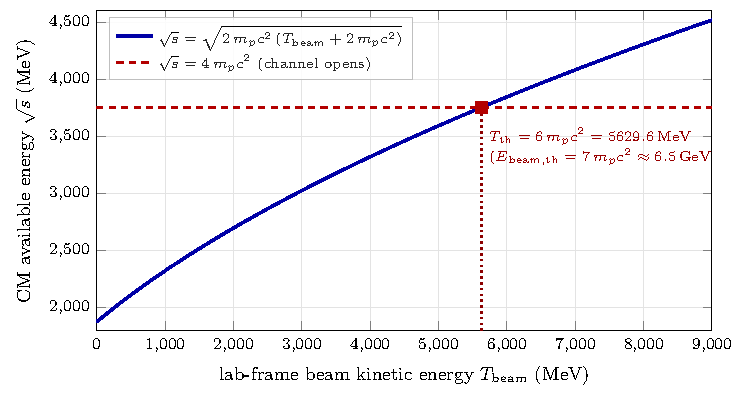
\includegraphics[width=0.86\linewidth]{figures/fig06_pair_threshold.pdf}
\caption{Fixed-target pair production: CM available energy
$\sqrt{s}=\sqrt{2\,m_pc^2(T_{\mathrm{beam}}+2\,m_pc^2)}$ (blue) versus
lab-frame beam kinetic energy. The $\bar p$-creation channel
$p+p\to p+p+\bar p+p$ opens when $\sqrt{s}$ first reaches $4\,m_pc^2$
(red dashed, the four final-nucleon rest energy). The intersection is the
registered verify anchor (red square): $T_{\mathrm{th}}=6\,m_pc^2=5629.6$\,MeV
beam kinetic, equivalently $E_{\mathrm{beam,th}}=7\,m_pc^2\approx6.5$\,GeV ---
the classic Bevatron number \citep{chamberlain1955}. Only the exact kinematic
curve and the single registered anchor are plotted; no experimental
cross-section points are invented (commons @D~g3). Atoms
\texttt{pair\_threshold\_kinetic} / \texttt{pair\_threshold\_total}
(\tierGreen) and \texttt{pair\_threshold\_factor}=6 /
\texttt{pair\_threshold\_total\_factor}=7 (\tierBlue, BLUE-MAX).}
\label{fig:prod-threshold}
\end{figure}

% -------------------------------------------------------------------------
\subsection{Verify atoms and verbatim verdicts}
\label{app:prod-verify}

Three families of atoms close process \textcircled{\scriptsize 1}: the
integer factors $6$ and $7$ (\tierBlue), and the two dimensional threshold
energies at $m_pc^2=938.272$\,MeV (\tierGreen). Their verbatim ledger rows
are in Table~\ref{tab:prod-verify}.

\begin{table}[h]
\centering
\small
\setlength{\tabcolsep}{5pt}
\begin{tabular}{@{}l l r r r l@{}}
\toprule
\textbf{atom} & \textbf{args} & \textbf{expected} & \textbf{observed} & $|\Delta|$ & \textbf{tier} \\
\midrule
\verb|pair_threshold_factor|        & (1)       & $6$       & $6$       & $0$        & \tierBlue \\
\verb|pair_threshold_kinetic|       & (938.272) & $5629.63$ & $5629.63$ & $9.1\times10^{-13}$ & \tierGreen \\
\verb|pair_threshold_total|         & (938.272) & $6567.9$  & $6567.9$  & $0$        & \tierGreen \\
\verb|pair_threshold_kinetic_factor|& ()        & $6$       & $6$       & $0$        & \tierBlue \\
\verb|pair_threshold_total_factor|  & ()        & $7$       & $7$       & $0$        & \tierBlue \\
\bottomrule
\end{tabular}
\caption{Process \textcircled{\scriptsize 1} verify atoms
(\texttt{companion/verify-ledger.json}, PR~\#1014 dimensional, \#1094 BLUE-MAX
integer factors). The three \tierBlue\ integer atoms attest the exact factors
$6$ (kinetic) and $7$ (total) of Eq.~\eqref{eq:prod-result}; the two
\tierGreen\ atoms attest the dimensional values at the CODATA-2018 proton
rest energy.}
\label{tab:prod-verify}
\end{table}

\begin{lstlisting}
verify --expr pair_threshold_kinetic(938.272)=5629.63
  calc   = 5629.63 ~ expected 5629.63 (|Delta|=9.09e-13 <= eps=1e-9)
  tier   = SUPPORTED-NUMERICAL (hexa-native libm-class recompute)
verify --expr pair_threshold_total(938.272)=6567.9
  calc   = 6567.90 ~ expected 6567.9 (|Delta|=0.0 <= eps=1e-9)
  tier   = SUPPORTED-NUMERICAL (hexa-native libm-class recompute)
verify --expr pair_threshold_factor(1)=6
  calc   = 6 == expected 6 (|Delta|=0)
  tier   = SUPPORTED-FORMAL (integer algebraic-root identity)
\end{lstlisting}

% -------------------------------------------------------------------------
\subsection{Honest scope}
\label{app:prod-scope}

This appendix closes the \emph{threshold} --- the exact beam energy below
which no antiproton can be made --- not the production \emph{yield}. The
yield above threshold is governed by the energy-dependent production
cross-section $\sigma_{p\bar p}(E)$ and the target thickness; both are
beam-line and detector inputs out of scope here, and no cross-section value
is claimed or plotted (commons @D~g3). The number this funnel asserts is the
kinematic gate, which is exact integer kinematics and which the Bevatron
confirmed historically by producing the first antiprotons at exactly this
$\sim$6.5\,GeV design energy \citep{chamberlain1955}.
